\documentclass[11pt,twoside]{article}
\usepackage[spanish, es-tabla]{babel}
\usepackage[utf8]{inputenc}
\usepackage{booktabs}
\usepackage{booktabs}     % tablas 
\usepackage{tabulary}     % tablas
\usepackage{graphicx}      % poner imagenes 
\usepackage{float}         % para fijar las imagenes con h y H
\usepackage{fancyhdr}
% Margins
\topmargin 0.02cm
\headheight 0.02cm
\textwidth 15.50cm
\oddsidemargin .0in
\evensidemargin .0in

\date{}

\begin{document}


	
\fancypagestyle{firststyle}
{
	\fancyhead[R]{ \tiny{Facultad de Ciencias, Facultad de Minas \\
			Universidad Nacional de Colombia, Sede Medellín\\
			2019}}
	\fancyhead[L]{}
	\fancyfoot[LO,RE]{}
	\fancyfoot[LE,RO]{ \vspace{10pt}\thepage}
	\renewcommand{\headrulewidth}{0pt}
	\renewcommand{\footrulewidth}{0pt}
}

\thispagestyle{firststyle}
\begin{center}
	\Large{{\bf STATISOFT 2.0\\
			\vspace{20pt}  PREDICCIÓN DEL NIVEL DE SATISFACCIÓN DE LAS MADRES SOLTERAS EN COLOMBIA\\ 
			\vspace{10pt}}}
\end{center}

{\normalsize{
		Heber Esteban Bermúdez			\footnote{\footnotesize{ hebermudezg@unal.edu.co}}
		John Bryan Yepez				\footnote{\footnotesize{ jbyepezh@unal.edu.co}},
		Simon Zapata 					\footnote{\footnotesize{sizapatagu@unal.edu.co}},
		Nelson Ordónez 			\footnote{\footnotesize{neordoñezm@unal.edu.co}}
}}




\begin{abstract}
\noindent
El presente proyecto pretende conocer cuáles son los factores que más afectan el nivel de satisfacción las madres solteras en Colombia y también crear una aplicación web para predecir este nivel de satisfacción. Para conocer este fenómeno el grupo de trabajo \textbf{Statisoft 2.0} empleo datos abiertos del Departamento Administrativo Nacional de Estadística \textbf{(DANE)} de la Encuesta de Calidad de Vida del año 2017 y usando técnicas estadísticas con los software \textbf{R} y el paquete Shinny crea un modelo estadístico y una aplicación de uso público que logra predecir el cómo se comporta satisfacción de las madres solteras usando las algunas de las variables de la encuesta, es por eso que el grupo \textbf{StatiSoft 2.0} crea un entendimiento a partir de los conceptos amplios como calidad de vida y madre soltera para desenlazar con el desarrollo de la aplicación. \\
\textbf{Palabras Clave}: satisfacción personal, calidad de vida, madre soltera.
\end{abstract}



%***-------------------------------------INTRODCUCCION-----------------------------------------------------
\section{Introducción}
\noindent
La calidad de vida es un concepto de amplio bagaje que se ha tratado desde hace un tiempo en Colombia debido a la estratificación socio-económica. La calidad de vida hace alusión a cinco áreas distintas como lo son: Bienestar físico, bienestar material, bienestar social, desarrollo y bienestar emocional; siendo este último uno de los factores psicológicos mas importantes para la satisfacción con la calidad de vida y el desarrollo de las otras cuatro áreas. La satisfacción con la vida busca e intenta definir  que es una buena vida y evaluar lo bien que vivimos, aunque aún así siga siendo un juicio subjetivo, cada persona está supeditada a encontrar su punto de equilibrio para decir que tan satisfecha está con su vida.
\\
\\
\noindent
El nivel de satisfacción de la vida es una apreciación subjetiva que aporta al bienestar general, ya que permite evaluar de manera personal cómo va tu vida en relación a lo que esperas de ella; por eso esta definición juega un papel muy importante en los hogares colombianos. Según el diario El Heraldo, para el 2017 había 22 millones de mujeres en el país, de las cuales sólo el 41,9{\%} tienen una ocupación formal o informal fuera del hogar y según datos del DANE, el 56{\%} de esas 22 millones de mujeres son cabeza de familia, es decir, madres solteras. Por lo anterior, se evidenca diferencia marcada tanto de madres solteras como de la crítica desventaja en términos laborales entre hombres y mujeres.
\\
\\
\noindent
Con el objetivo de mostrar el nivel de satisfacción de las madres solteras en Colombia, la Encuesta de Calidad de Vida del 2017 publicada por el DANE es la materia prima principal para responder la pregunta planteada: ¿Qué afecta la satisfacción de las madres solteras? Además, a la persona interesada le permite saber cuál es el nivel de satisfacción de la madre soltera según los esquemas de preguntas formulados por el DANE, los cuales en el presente trabajo son tratados como variables. Dicha Encuesta de Calidad de Vida fue formulada a través de un diseño muestral probabilístico, estratificado, multietpico, de conglomerados.
\\
\\
\noindent
Ante esta duda de cuál es el nivel de satisfacción de las madres solteras y qué factores influyen, es creada la aplicación StatiSoft, la cual tiene un desarrollo que podrá predecir el nivel de satisfacción de las madres solteras en función de variables como la percepción de satisfacción en cuanto al ingreso económico, salud, seguridad, felicidad, tranquilidad, número de hijos, número de nietos, acceso a internet y uso de redes sociales, para así predecir su nivel de satisfacción con la vida. 
\\
\\
Esta aplicación es de  uso abierto y  baja complejidad por lo que a empresas y personas particulares  se les facilitará usarlo, ademas de ser fundamental para promover la investigación sobre las condiciones de vida y la medición de la pobreza en los hogares colombianos, donde las poblaciones más afectadas son las madres solteras que no cuentan con ayuda para la crianza de sus hijos y el manejo del hogar.




%***------------------------------------------DEFINICIONES-----------------------------------------------
\section{Definiciones}
\noindent
A continuación se definen claramente los conceptos tratados en nuestro estudio y desarrollo del trabajo \\
\\
\textbf{Madre soltera} \\
Se denomina madre soltera generalmente a un tipo de familia monoparental, en la que una mujer lleva a cabo la crianza de los hijos y el manejo del hogar sin la compañía o apoyo de una pareja, por decisión propia o circunstancias de su entorno. En un sentido muy estricto se podría hablar con propiedad de núcleo familiar monoparental cuando el conjunto es formado por un progenitor (madre o padre, en este caso madre) y uno o varios hijos. Este núcleo puede constituir por sí solo una familia independiente (familia nuclear monoparental), o puede convivir con otras personas emparentadas. Por ejemplo, una madre (sin pareja) con dos hijos que convivan con sus padres constituye un núcleo monoparental en una familia extensa. Debido a esto no se excluyen el número de personas con las que viva la madre soltera.\\
En conclusión, para nuestro estudio hemos tomado la mujeres solteras y viudas de cualquier edad que tiene uno o más hijos en el hogar.\\
\\
\textbf{Nivel de satisfacción con la vida}\\
La satisfacción con la vida es una apreciación subjetiva que aporta al bienestar general, ya que permite evaluar de manera personal cómo va tu vida en relación con lo que esperas de ella. Tratar este tipo de temas resulta algo denso y complicado ya que la categorización de este requiere un análisis agudo según la satisfacción que tenga la persona con diferentes factores que pueden alterar su entorno y vida diaria.\\
Para la Organización Mundial de la Salud, ésta última refiere no sólo al estado completo de bienestar físico y mental sino también social y dado una fase tan subjetiva, el tipo de análisis comienza desde un aspecto psicológico.



%***------------------------------------------ ANALISIS-----------------------------------------------------

%\section{Análisis}

El objetivo principal del proyecto es 




%***---------------------------------------- METODOLOGIA-----------------------------------------------------

\section{Metodología}
\noindent
En la primera etapa del desarrollo del trabajo fue preciso hacer un análisis descriptivo previo, para observar el comportamiento de las posibles variables significativas para el modelo, y luego adoptar la metodología estadística a implementar (ver sección 3.1) para crear el modelo que permita hacer la correcta predicción del nivel de satisfacción de las madres solteras en Colombia. Para el estudio se usaron los datos de la encuesta nacional de calidad de vida del \textbf{DANE}, donde se seleccionaron las mujeres que cumplieran con las características de tener uno o más hijos y que fueran solteras o viudas esto acorde con la definición mencionada (ver sección \textbf{2. Definiciones}).
\\
Nuestro estudio se enfocó en analizar cómo las variables de características y composición del hogar y el acceso a tecnologías de información y comunicación afecta el nivel de vida de las madres solteras, en primera instancia para el análisis estadístico se realiza un análisis descriptivo de la base de datos, obteniendo como resultado una depuración de observaciones que no brindan información relevante para la estimación del nivel se satisfacción de vida, se realiza una limpieza de datos eliminando las observaciones que presentaban información faltante (NA) en nuestras variables a analizar, posteriormente se hace el análisis del modelamiento estadístico, se describe claramente como se realizo este, y por último se hace un análisis diagnostico del modelo para evaluar la calidad del mismo. 
\\
\subsection{Análisis descriptivo}
\noindent
En la Tabla 1 se muestra la dimensión del conjunto de datos analizados para este proyecto, donde se tiene un total de 901 registros y 24 variables.
%**-------------------- Tabla 1 -----------
\begin{table}[H]
	\caption{\small{Dimensión de la base de datos.}}
	\label{tabla1}
	\centering {\small
		
	\begin{tabular}{@{}cc@{}}
		\toprule
		Número de Filas & Número de Columnas \\ \midrule
		901             & 24                 \\ \bottomrule
	\end{tabular}}
\end{table}
Cada registro corresponde a una madre soltera acorde con la definición mencionada (ver sección\textbf{ 2. Definiciones}) y cada columna corresponde a una variable medida en la madre soltera en aspectos de estructura del hogar al que pertenece y acceso a tecnologias de información y la comunicación. 

\paragraph{Descripción de las variables:} a continuación se muestran una descripción de las variables medidas para cada madre soltera (ver Tabla 2). 
\begin{table}[H]
	\caption{\small{Descripción de la variables medidas a las madres solteras.}}
	\label{tabla2}
	\centering {\small
	\begin{tabular}{@{}llll@{}}
		\toprule
		Variable & Descripción & Variable & Descripción \\ \midrule
		P6040 & Edad  en años & P1903 & \begin{tabular}[c]{@{}l@{}}Qué tan preocupada se sintió ayer\\ (del 0 al 10)\end{tabular} \\
		P5502 & Casada o Viuda & P1904 & \begin{tabular}[c]{@{}l@{}}Qué tan triste se sintió ayer \\ (del 0 al 10)\end{tabular} \\
		P6081 & \begin{tabular}[c]{@{}l@{}}El padre vive en el hogar\\  (si o no)\end{tabular} & P1905 & \begin{tabular}[c]{@{}l@{}}Qué tanto considera que las cosas\\  que hace en su vida valen la pena \\ (del 0 al 10)\end{tabular} \\
		P6083 & \begin{tabular}[c]{@{}l@{}}La madre de vive en el hogar\\ (si o no)\end{tabular} & N\_HIJOS & Número de hijos \\
		P6080 & \begin{tabular}[c]{@{}l@{}}Se reconoce como (Indegena, Gitano, \\ Raizal, Palenquero, Negro o \\ ninguno de los anteriores)\end{tabular} & N\_NIETOS & Número de nietos \\
		P1895 & \begin{tabular}[c]{@{}l@{}}Que tan satisfecha se siente con su vida\\ (Variable Respuesta)\end{tabular} & P1910 & \begin{tabular}[c]{@{}l@{}}Frecuencia con la que utiliza\\ computador de escritorio\end{tabular} \\
		P1896 & \begin{tabular}[c]{@{}l@{}}Qué tan satisfechoa se siente con su ingreso\\ (del 0 al 10)\end{tabular} & P1911 & \begin{tabular}[c]{@{}l@{}}Frecuencia con la utiliza\\ computador portatil\end{tabular} \\
		P1897 & \begin{tabular}[c]{@{}l@{}}Qué tan satisfecha se siente con su salud\\  ( del 0 al 10)\end{tabular} & P1912 & \begin{tabular}[c]{@{}l@{}}Frecuencia con la que\\ utiliza tableta\end{tabular} \\
		P1898 & \begin{tabular}[c]{@{}l@{}}Qué tan satisfecha se siente con\\ su nivel de seguridad ( del 0 al 10)\end{tabular} & P1084 & \begin{tabular}[c]{@{}l@{}}Frecuencia con la que\\  utiliza internet\end{tabular} \\
		P1899 & \begin{tabular}[c]{@{}l@{}}Qué tan satisfecha se siente con su\\ trabajo/actividad (del 0 al 10)\end{tabular} & P1083S3 & Usa redes sociales (si o no) \\
		P1901 & \begin{tabular}[c]{@{}l@{}}Qué tan feliz se sintió ayer\\  (del 0 al 10)\end{tabular} & P1082 & Tiene teléfono celular (si o no) \\
		P1902 & \begin{tabular}[c]{@{}l@{}}Qué tan tranquila se sintió ayer \\ (del 0 al 10)\end{tabular} & P804 & \begin{tabular}[c]{@{}l@{}}Frecuencia con la que escucha\\ señal de radio\end{tabular} \\ \bottomrule
	\end{tabular}}
\end{table}


\textbf{Análisis descriptivo de la variable respuesta:} en la Figura 1 se muestra un diagrama de de barras donde se aprecia una asimetría de la frecuencia, esto es un sesgo a la izquierda en la distribución del nivel de satisfacción, del mismo modo se puede notar que la mayor parte de las madres solteras tiene una satisfacción superior a seis (6). 
\\
\begin{figure}[H]
	\centering
	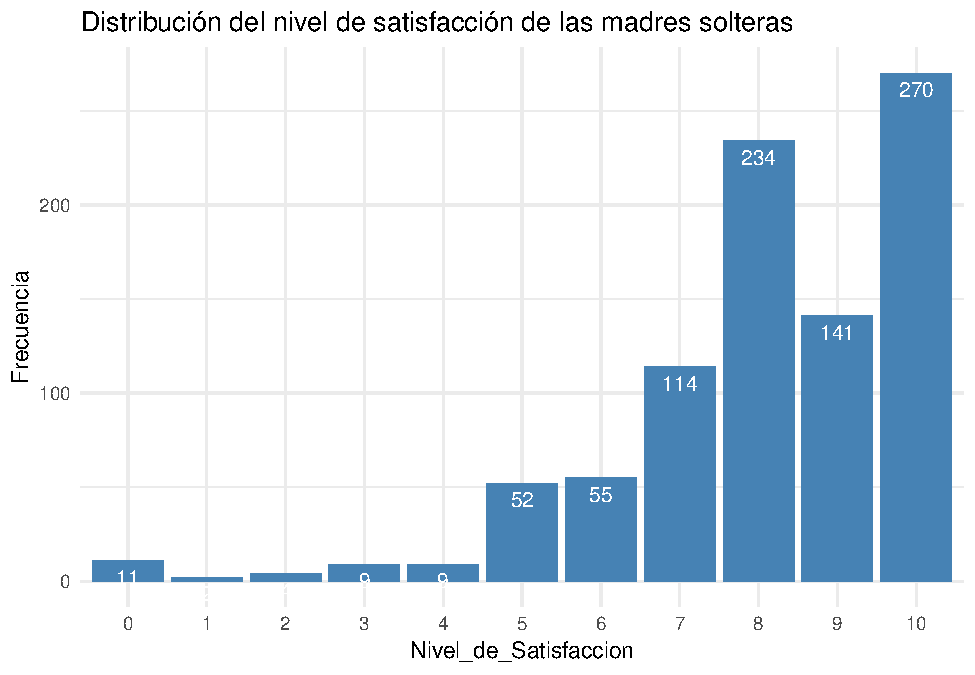
\includegraphics{barras2.pdf}
	\caption{Diagrama de barras, distribución de la satisfacción de las madres solteras}
\end{figure}



\vspace{100px}
\noindent
En la Figura 2 se muestra el diagrama de caja y bigotes de la distribución de la variable respuesta donde se puede observar que el un 75{\%} de las madres solteras tiene un nivel de satisfacción superior al nivel 7. 
\begin{figure}[H]
	\centering
	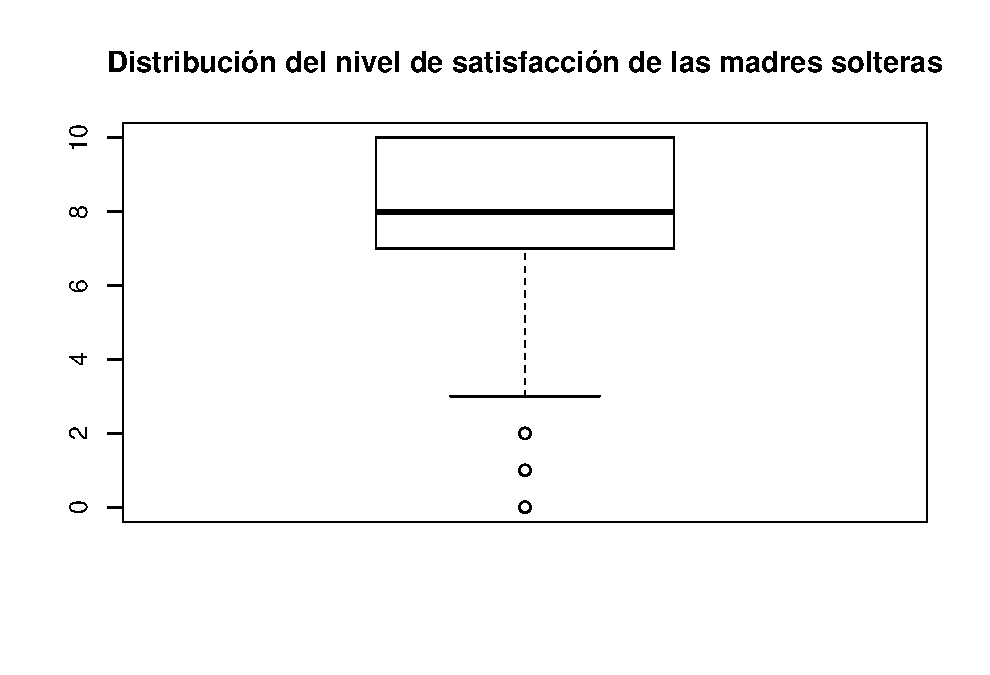
\includegraphics{boxplot1.pdf}
	\caption{Diagrama de caja y bigotes (boxplot) de la distribución de la satisfacción de las madres solteras}
\end{figure}
% hace falta porner otros graficoss****


\vspace{120px}
\noindent
En la Figura 3 se muestra un gráfico de barras de la distribución del número de hijos de las madres solteras, se puede observar claramente que la existen 557 madres que tienen 1 solo hijo, mientras que apenas existen 7 mujeres con 5 hijos.  
\begin{figure}[H]
	\centering
	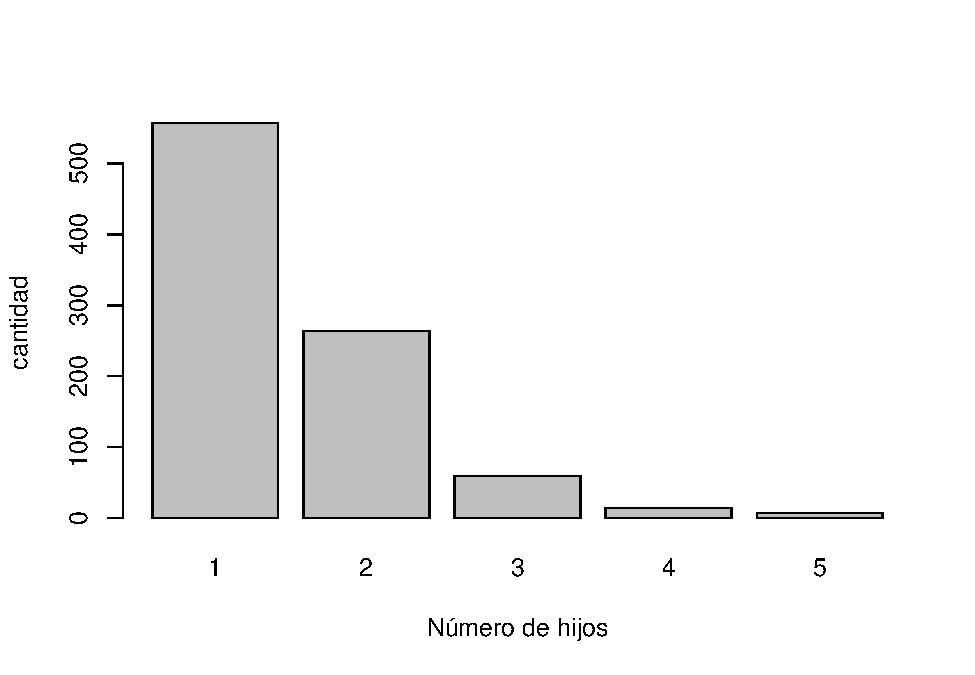
\includegraphics{barrasnumerodehijos.pdf}
	\caption{Distribución de la cantidad de hijos de las madres solteras}
\end{figure}

\vspace{140px}
\noindent
En la Figura 4 se muestra un gráfico de barras que muestra la distribución del número de nietos de la madre soltera, donde se observa que la mayoría de las madres solteras no tienen nietos aún.
\begin{figure}[H]
	\centering
	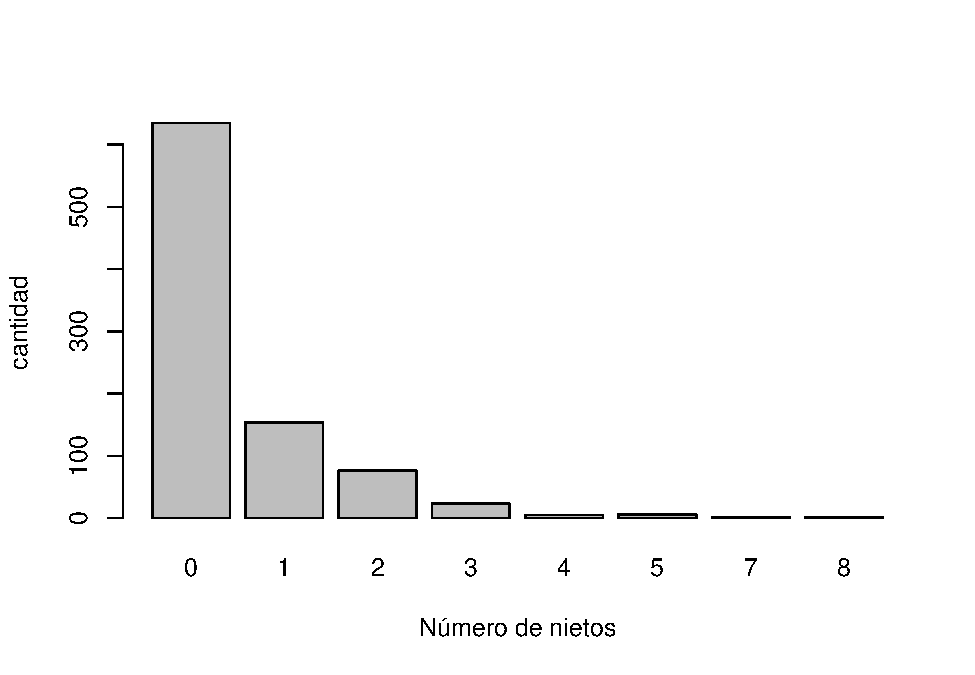
\includegraphics{barrasnumerodenietos1.pdf}
	\caption{Distribución de la cantidad de nietos de las madres solteras}
\end{figure}

\vspace{140px}
\noindent
En la Figura 5 se muestra la distribución del uso de las redes sociales donde ser puede observar que la mayor parte de las madres solteras no hacen uso de esta herramienta.
\begin{figure}[H]
	\centering
	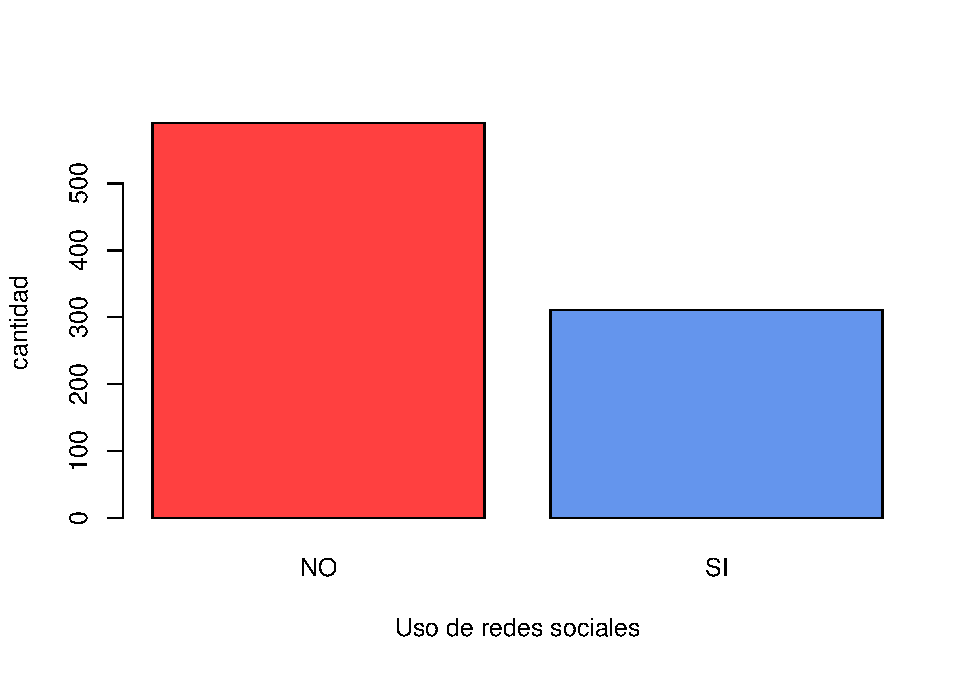
\includegraphics{usoderedes.pdf}
	\caption{Distribución del uso de la redes sociales}
\end{figure}



\subsection{Modelamiento estadístico}
\noindent
Se decidió implementar un modelo de regresión logística multinomial, metodología enmarcada en los modelos lineales generalizados\textbf{ (MLG)} que permite más de dos posibles resultados para la variable respuesta de tipo categórico ordinal. 
\\
Antes de realizar el modelo multinomial se realizó un modelo de regresión lineal múltiple (suponiendo la variable respuesta como cuantitativa) para evaluar el proceso de selección de variables, este procedimiento se desarrolló haciendo uso función stepGAIC() de la librería MASS en el software estadístico R, lo cual permite usar un procedimiento de selección de variables hacia adelante (forward) y hacia atrás (backward), definiendo como frontera del modelo la combinación lineal de todas las variables explicativas categóricas (ya convertidas en factores, variables dummy) como también la interacción sencilla entre las variables explicativas cuantitativas.
Las variables seleccionadas con la función stepGAIC() y parámetro (direction=’both’) que me permite hacer selección de variables en ambas direcciones.








\subsection{Diagnóstico del Modelo}








%***-----------------------------------------CONCLUCIONES--------------------------------------------------
\section{Conclusiones}







%***----------------------------------------APLICACION WEB--------------------------------------------
\section{Aplicación web}






%***----------------------------------------REFERENCIAS--------------------------------------------
\section{Referencias}
[1] El estudio de la satisfacción con la vida, Ruut Veenhoven 
[2] Problemas que debe enfrentar una madre soltera - https://madresoltera.org/problemas/
[3] 

\end{document}